\documentclass{beamer}

%% Juego de caracteres usado en el archivo fuente: UTF-8
\usepackage{ucs}
\usepackage[utf8x]{inputenc}
\uselanguage{spanish}
%Para la identación del español
\usepackage[spanish]{babel}
\usepackage{animate}

% There are many different themes available for Beamer. A comprehensive
% list with examples is given here:
% http://deic.uab.es/~iblanes/beamer_gallery/index_by_theme.html
% You can uncomment the themes below if you would like to use a different
% one:
%\usetheme{AnnArbor}
%\usetheme{Antibes}
%\usetheme{Bergen}
%\usetheme{Berkeley}
%\usetheme{Berlin}
%\usetheme{Boadilla}
%\usetheme{boxes}
%\usetheme{CambridgeUS}
%\usetheme{Copenhagen}
%\usetheme{Darmstadt}
%\usetheme{default}
%\usetheme{Frankfurt}
%\usetheme{Goettingen}
%\usetheme{Hannover}
%\usetheme{Ilmenau}
%\usetheme{JuanLesPins}
%\usetheme{Luebeck}
\usetheme{Madrid}
%\usetheme{Malmoe}
%\usetheme{Marburg}
%\usetheme{Montpellier}
%\usetheme{PaloAlto}
%\usetheme{Pittsburgh}
%\usetheme{Rochester}
%\usetheme{Singapore}
%\usetheme{Szeged}
%\usetheme{Warsaw}

%Para la identación del español
\usepackage[spanish]{babel}

\title{Inmovilizado}

% A subtitle is optional and this may be deleted
%\subtitle{Optional Subtitle}

\author{Jesús Rodríguez Heras \\ Juan Pedro Rodríguez Gracia \\ Gabriel Fernando Sánchez Reina}
% - Give the names in the same order as the appear in the paper.
% - Use the \inst{?} command only if the authors have different
%   affiliation.

%\institute[Escuela Superior de Ingeniería] % (optional, but mostly needed)
%{
%  \inst{1}%
%  Department of Computer Science\\
%  University of Somewhere
%  \and
%  \inst{2}%
%  Department of Theoretical Philosophy\\
%  University of Elsewhere}
% - Use the \inst command only if there are several affiliations.
% - Keep it simple, no one is interested in your street address.

%\date{8 de mayo de 2018}
% - Either use conference name or its abbreviation.
% - Not really informative to the audience, more for people (including
%   yourself) who are reading the slides online

%\subject{Theoretical Computer Science}
% This is only inserted into the PDF information catalog. Can be left
% out. 

% If you have a file called "university-logo-filename.xxx", where xxx
% is a graphic format that can be processed by latex or pdflatex,
% resp., then you can add a logo as follows:

% pgfdeclareimage[height=0.5cm]{university-logo}{university-logo-filename}
% \logo{\pgfuseimage{university-logo}}

% Delete this, if you do not want the table of contents to pop up at
% the beginning of each subsection:
%\AtBeginSubsection[]
%{
%  \begin{frame}<beamer>{Índice}
%    \tableofcontents[currentsection,currentsubsection]
%  \end{frame}
%}

% Let's get started
\begin{document}

\begin{frame}
  \titlepage
%  \begin{center}
%  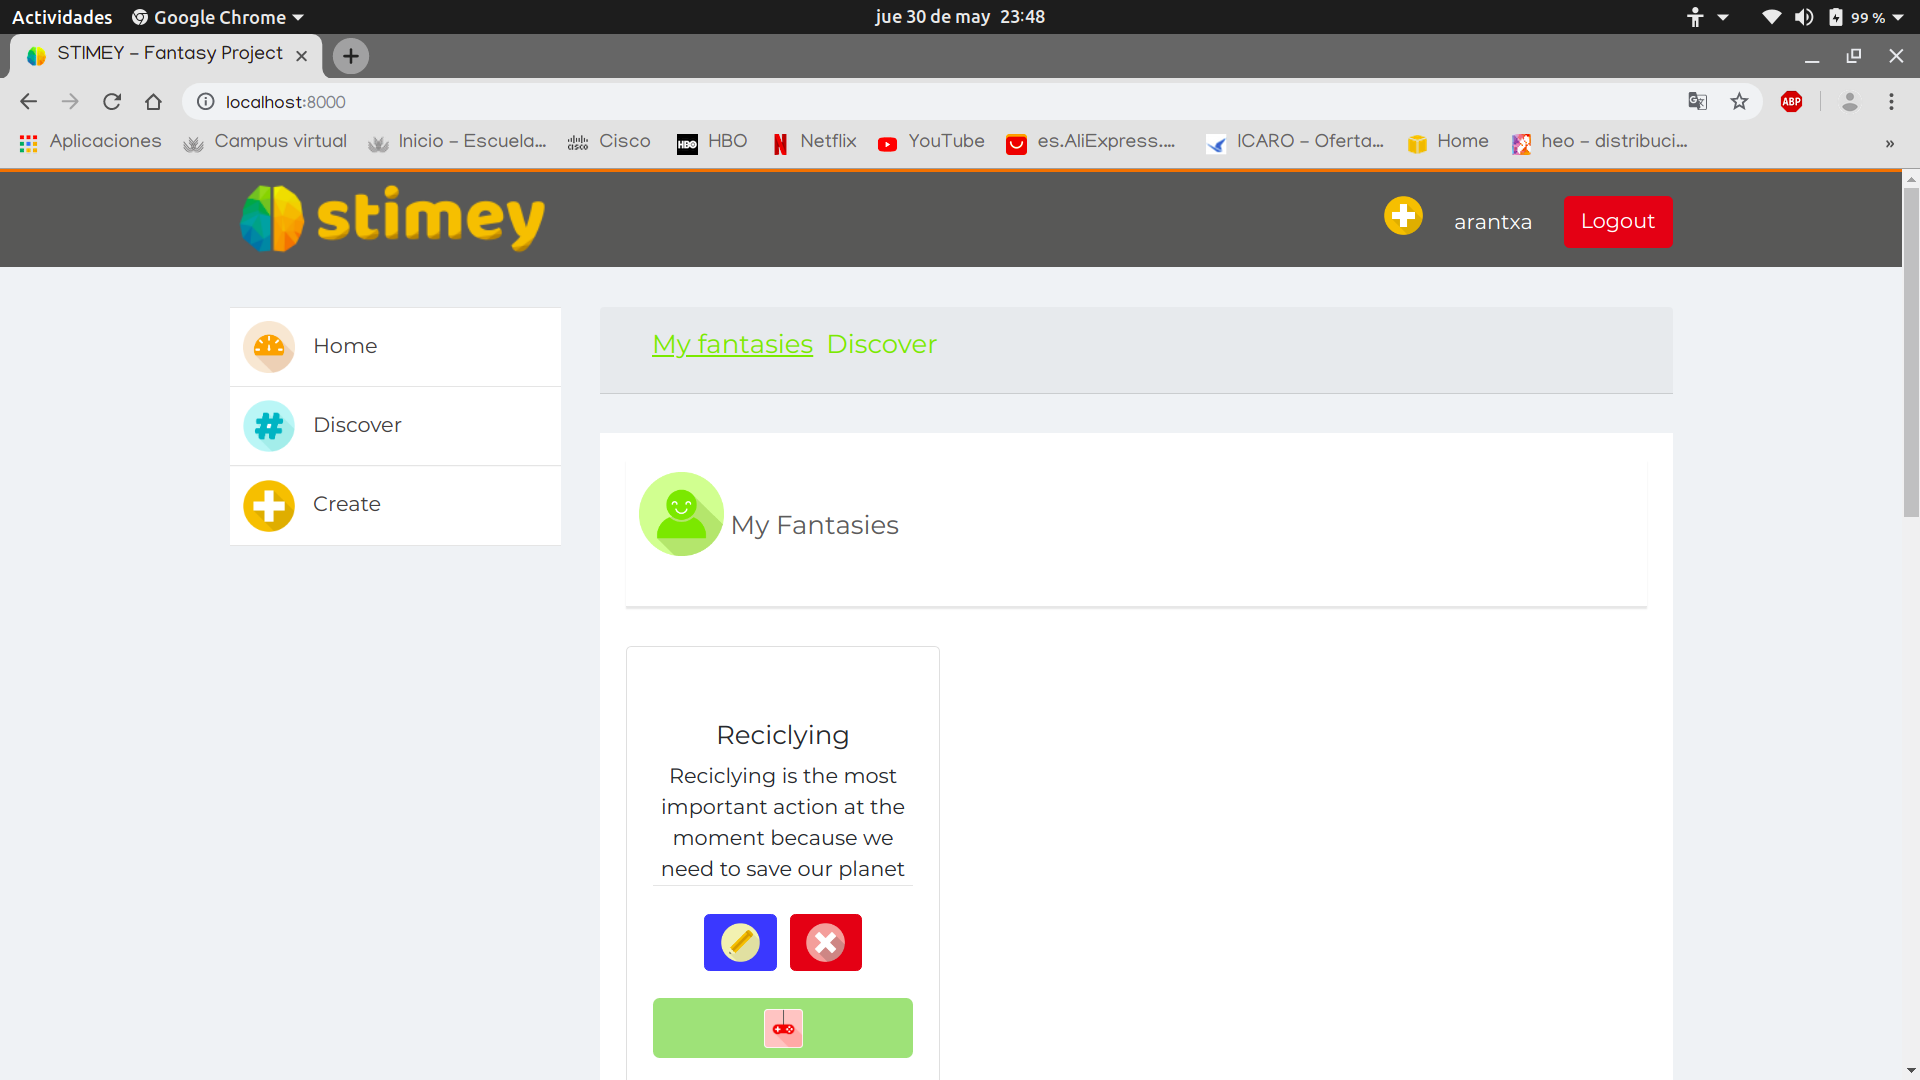
\includegraphics[scale=0.2]{Portada.png}	
%  \end{center}
  
\end{frame}

%\begin{frame}{Índice}
%  \tableofcontents
%  % You might wish to add the option [pausesections]
%\end{frame}

\begin{frame}{Inmovilizado}
	Hemos diseñado una base de datos correspondiente al excel que nos pasó nuestra compañera.\\
	También tenemos tres perfiles de usuario (auditor, supervisor y gerente) con sus respectivos permisos.
	\begin{itemize}
		\item Auditor: Select, Insert, Update y Delete.
		\item Supervisor: Select y Update.
		\item Gerente: Select.
	\end{itemize}
\end{frame}

\begin{frame}{Inmovilizado}
	Tenemos varios archivo en \texttt{.php}:
	\begin{itemize}
		\item \texttt{preSubir.php}.
		\item \texttt{Subir.php}.
		\item \texttt{generarhtml.php}.
		\item \texttt{menuSupervisor.php}.
		\item \texttt{supervisar.php}.
	\end{itemize}
\end{frame}

\begin{frame}{Problemas}
	Uno de los problemas fundamentales es que no tenemos una contabilidad, por lo que las pruebas que requieran comparar unos datos con otros, no podemos hacerlas a no ser que se haga manualmente por parte del auditor.
\end{frame}

\end{document}


